\documentclass{beamer}
\usepackage{xcolor}
\usepackage{natbib} % package to organize literature
\usepackage{multicol}
\usepackage{booktabs}
\usepackage{wasysym} % additional symbols
\usepackage{graphicx} % to include graphics, gifs
\usepackage{color} % add colored text
\usepackage{lmodern} % to fix font size error, might be problematic with math symbols
\usepackage{array}

\usetheme{Frankfurt}
\usecolortheme{beaver}
\setbeamertemplate{footline}
{
  \leavevmode%
  \hbox{%
  \begin{beamercolorbox}[wd=.3\paperwidth,ht=2.25ex,dp=1ex,center]{author in head/foot}%
    \usebeamerfont{author in head/foot}\insertshortauthor \hspace{1em} (\insertshortinstitute)
  \end{beamercolorbox}%
  \begin{beamercolorbox}[wd=.4\paperwidth,ht=2.25ex,dp=1ex,center]{title in head/foot}%
    \usebeamerfont{title in head/foot}\insertshorttitle
  \end{beamercolorbox}%
  \begin{beamercolorbox}[wd=.3\paperwidth,ht=2.25ex,dp=1ex,right]{author in head/foot}%
    \usebeamerfont{author in head/foot}\insertdate \hspace{2em}
    \insertframenumber{} / \inserttotalframenumber\hspace*{1em}
  \end{beamercolorbox}}%
  \vskip0pt%
}
%\definecolor{beamer@sbred}{rgb}{0.65,0.15,0.18}
\definecolor{beamer@sbred}{rgb}{0.22,0.22,0.66}
\setbeamercolor{title}{fg=beamer@sbred,bg=black!5}
\setbeamercolor{structure}{fg=beamer@sbred}
\setbeamercolor{frametitle}{fg=beamer@sbred}
\setbeamercolor{palette primary}{fg=beamer@sbred,bg=black!10}
\setbeamercolor{palette secondary}{fg=beamer@sbred}
\setbeamercolor{palette tertiary}{bg=beamer@sbred}
\setbeamercolor{palette quaternary}{fg=white,bg=beamer@sbred}
\setbeamertemplate{itemize items}[default]
\setbeamertemplate{enumerate items}[default]
\setbeamersize{text margin left=1em,text margin right=1em}
\DeclareTextFontCommand{\emph}{\color{beamer@sbred}}

\author[DeScioli \& Kraft]{Peter DeScioli \and Patrick Kraft}
\institute[Stony Brook]{73rd MPSA Conference}
\title[Should the Majority Rule?]{Should the Majority Rule?\\{\small When Majority Voting Leads to Suboptimal Choices}}
\date{April 17, 2015}
\titlegraphic{\includegraphics[width=4cm]{/data/Copy/1-src/logos/logo_bk.pdf}}

\begin{document}
\frame{\titlepage}
%\footnotesize


\section{Introduction}

\subsection{}
\begin{frame}%[allowframebreaks]
\frametitle{Questions}
\begin{itemize}
\item Is the majority rule \emph{efficient}?
\item How does its efficiency depend on how we \emph{conceptualize} individual preferences and utilities?
\end{itemize}
\end{frame}

\begin{frame}%[allowframebreaks]
\frametitle{Inefficient Majorities}
\begin{table}[c]
  \caption{Example for Inefficient Majorities}
  \begin{center}
    \begin{tabular}{lcc}
    \hline
     & \textbf{Policy 1} & \textbf{Policy 2} \\
    \hline
       Voter 1 & 10 & 100 \\
       Voter 2 & 110 & 100 \\
       Voter 3 & 110 & 100 \\
    \hline
    \end{tabular}
  \end{center}
\end{table}
    \emph{Conceptualization} of efficiency:
    \begin{itemize}
      \item Does the election result \emph{maximize the aggregated utilities} for all voters?
      \item $ \sum_i U_i^{W} \geq \sum_i U_i^{L} $
    \end{itemize}
\end{frame}

\subsection{}
\begin{frame}%[allowframebreaks]
\frametitle{Voting, Ideal Points, and Utilities}
\begin{itemize}
  \item \emph{Spatial theory of voting}\\\citep[e.g.][]{downs1957economic,enelow1984spatial}:
  \begin{itemize}
     \item common policy / ideological dimension
     \item utilities determined by relative \emph{proximity}
   \end{itemize}
  \begin{figure}[b]\centering
      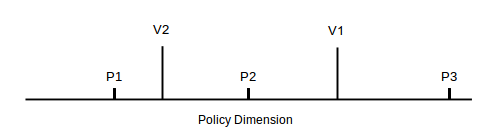
\includegraphics[width=.8\textwidth]{../paper/ideal_plot.png}
  \end{figure}
  \end{itemize}
  $$ U_{ij} = -(V_i - P_j)^2 $$
\end{frame}

\section{Simulation Results}
\subsection{}
\begin{frame}%[allowframebreaks]
  \frametitle{Simulation Scenarios}
  \begin{itemize}
    \item Overview:
    \begin{itemize}
      \item Number of \emph{voters} in each election: 2000
      \item Number of \emph{candidates} in each election: 2
      \item Number of \emph{simulations} for each scenario: 1000
      \item Individual \emph{utilities} based on ideal points or directly simulated from distributions; voters vote for the candidate that maximizes their utility
      \item \emph{Goal:} investigate the \emph{efficiency} of majority voting under varying assumptions about voter preferences (conceptualization, shape, etc.)
    \end{itemize}
  \end{itemize}
\end{frame}

\subsection{}
\begin{frame}%[allowframebreaks]
  \frametitle{Study 1: Direct versus Spatial Utilities I}
  \begin{figure}[ht]\centering
    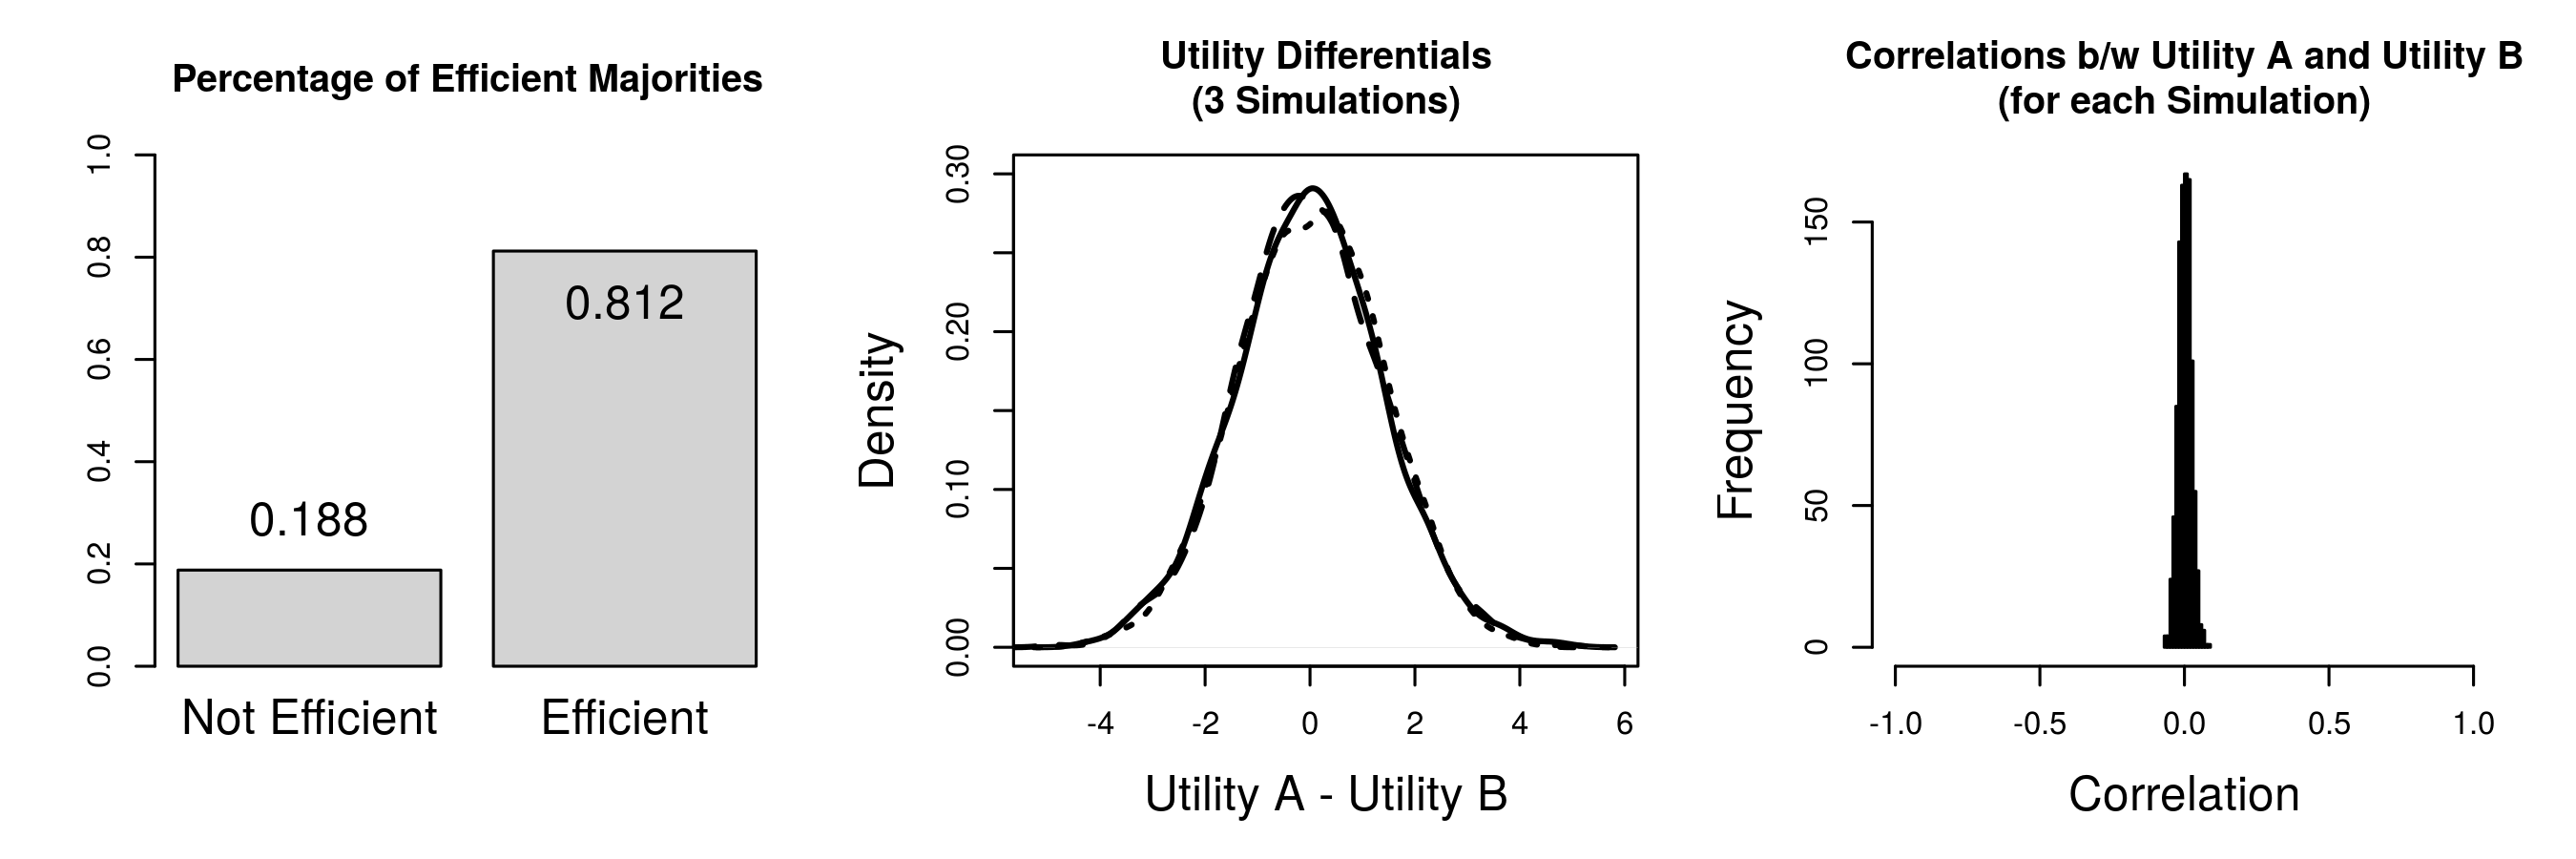
\includegraphics[width=\textwidth]{../simulations/fig/s1b.png}
    \caption{Direct preferences}
  \end{figure}
  $$ U_{ij} \sim \mathcal{N}(\mu=0,\sigma^2=1) $$
\end{frame}
\begin{frame}%[allowframebreaks]
  \frametitle{Study 1: Direct versus Spatial Utilities II}
  \begin{figure}[ht]\centering
    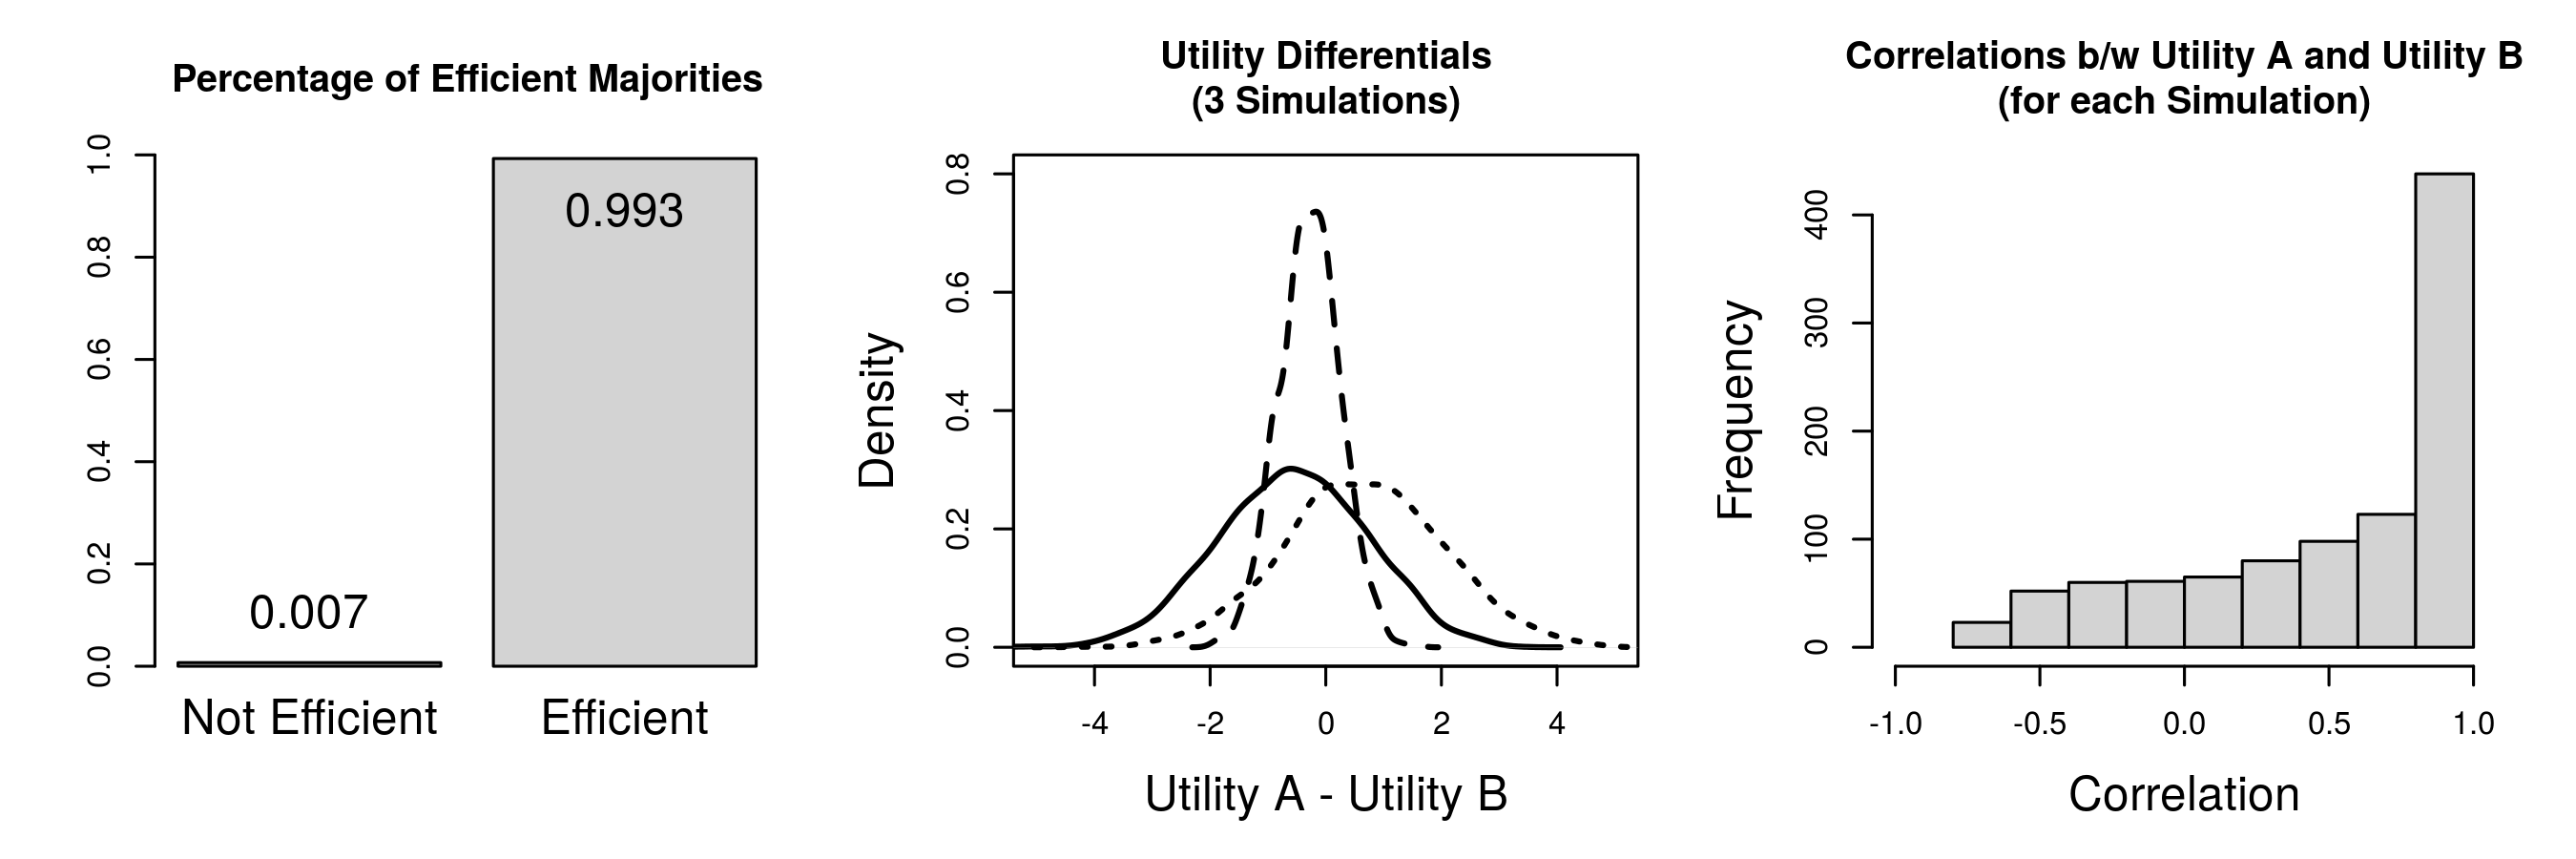
\includegraphics[width=\textwidth]{../simulations/fig/s1a.png}
    \caption{Spatial preferences}
  \end{figure}
  	$$ V_i,P_j \sim \mathcal{N}(\mu=0,\sigma^2=1) $$
	$$ U_{ij} = -(V_i - P_j)^2 $$
\end{frame}

\subsection{}
\begin{frame}%[allowframebreaks]
  \frametitle{Study 3: Mean Differences in Policy Utilities I}
  \begin{figure}[ht]\centering
    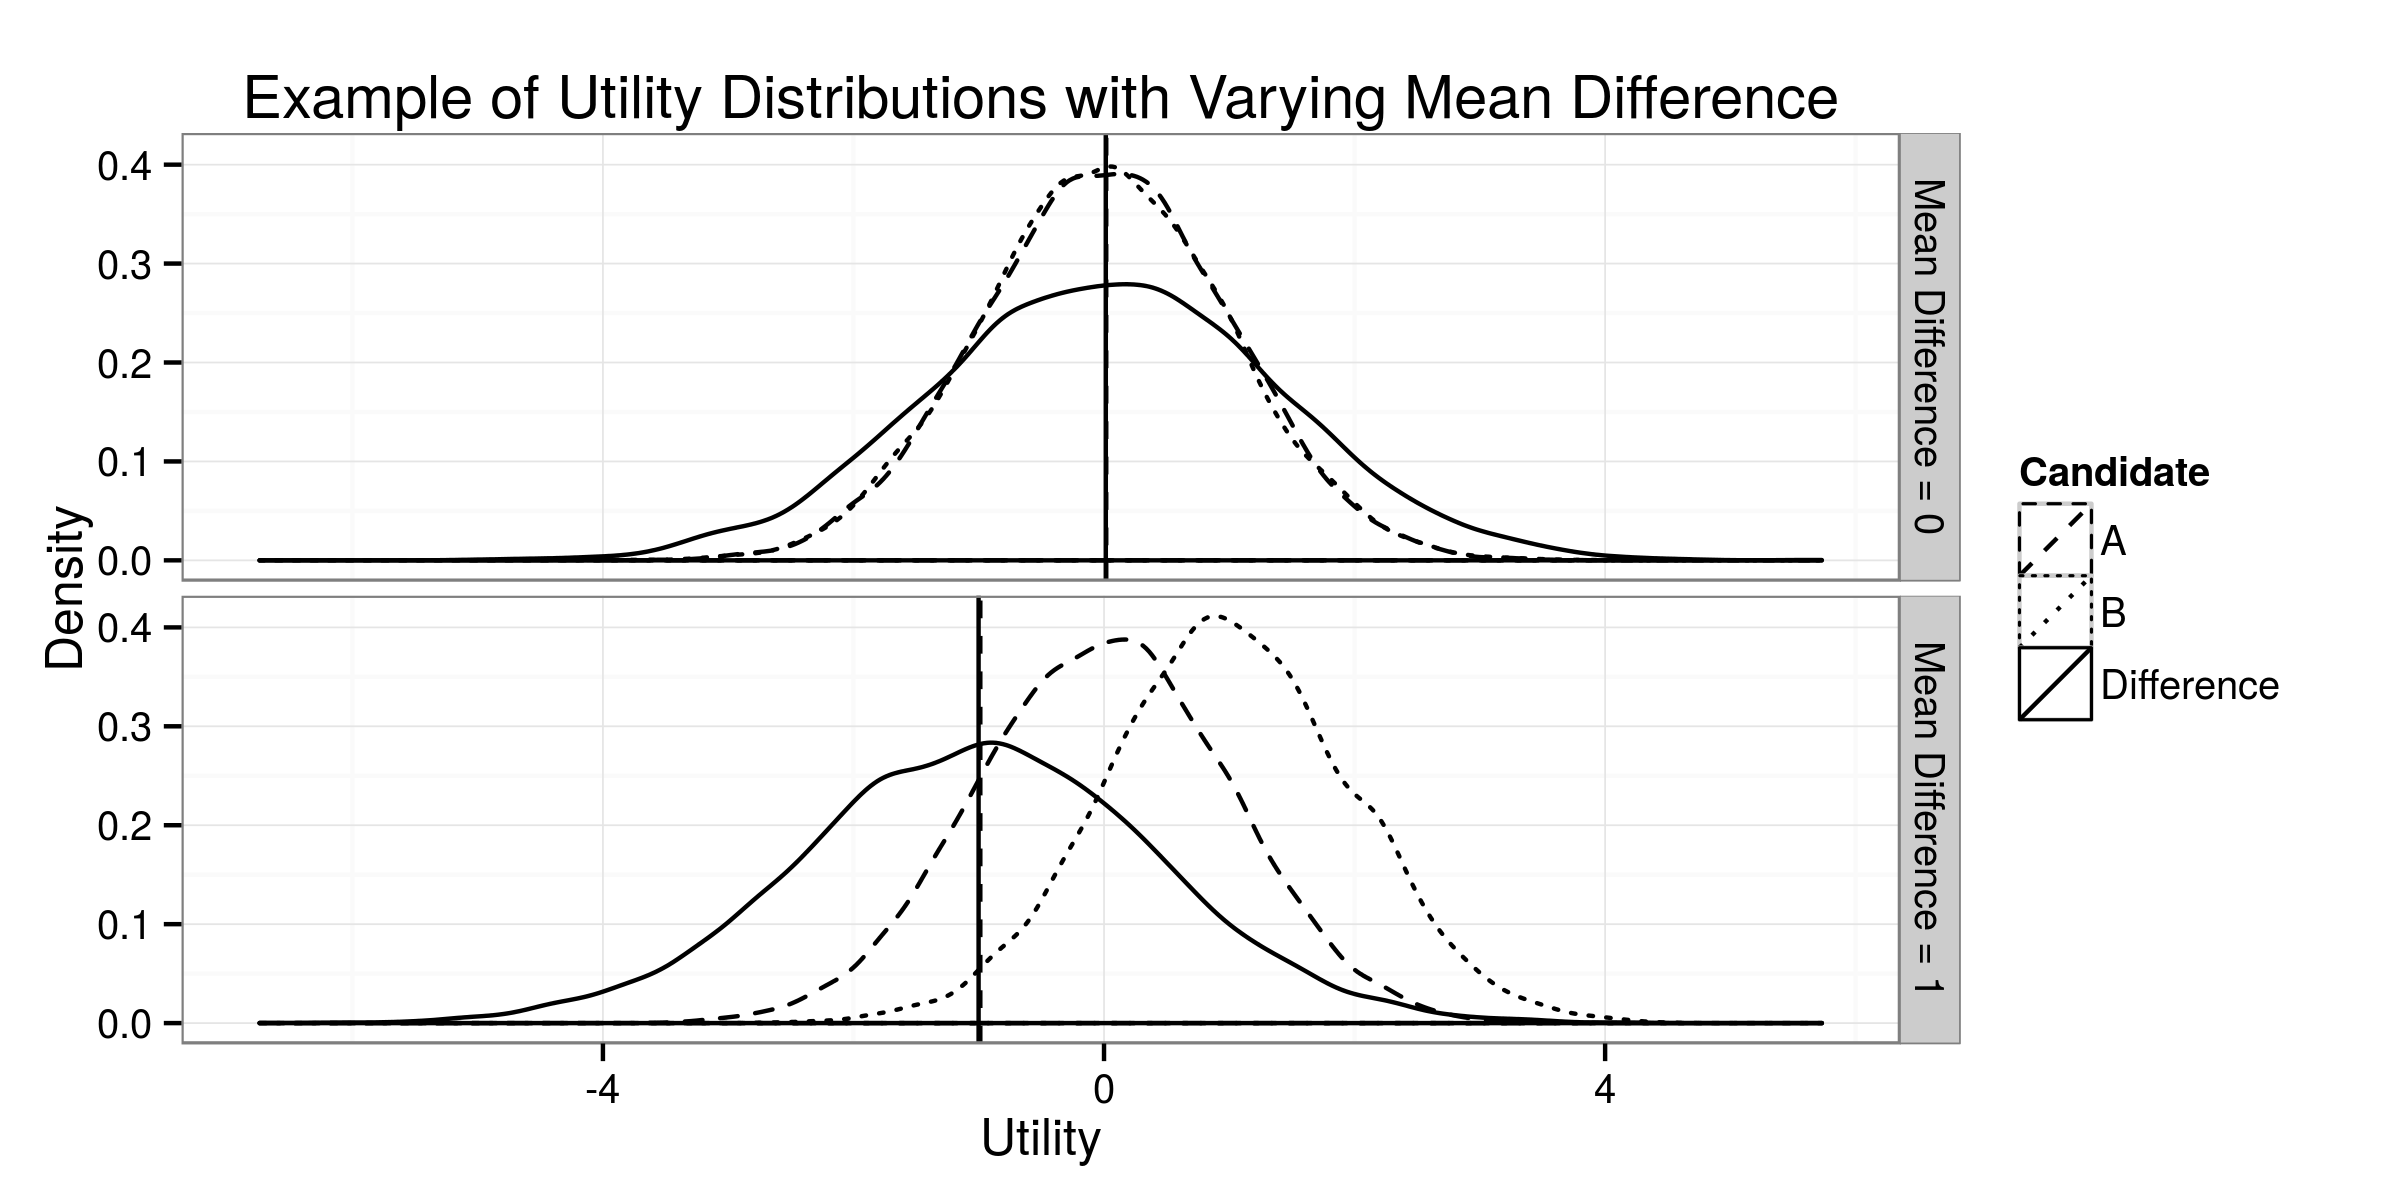
\includegraphics[height=.7\textheight]{../simulations/fig/s3a.png}
  \end{figure}
	$$ U_{i,A} \sim \mathcal{N}(\mu=0,\sigma^2=1) $$
        $$ U_{i,B} \sim \mathcal{N}(\mu=0+\epsilon,\sigma^2=1) $$
\end{frame}
\begin{frame}%[allowframebreaks]
  \frametitle{Study 3: Mean Differences in Policy Utilities II}
  \begin{figure}[ht]\centering
    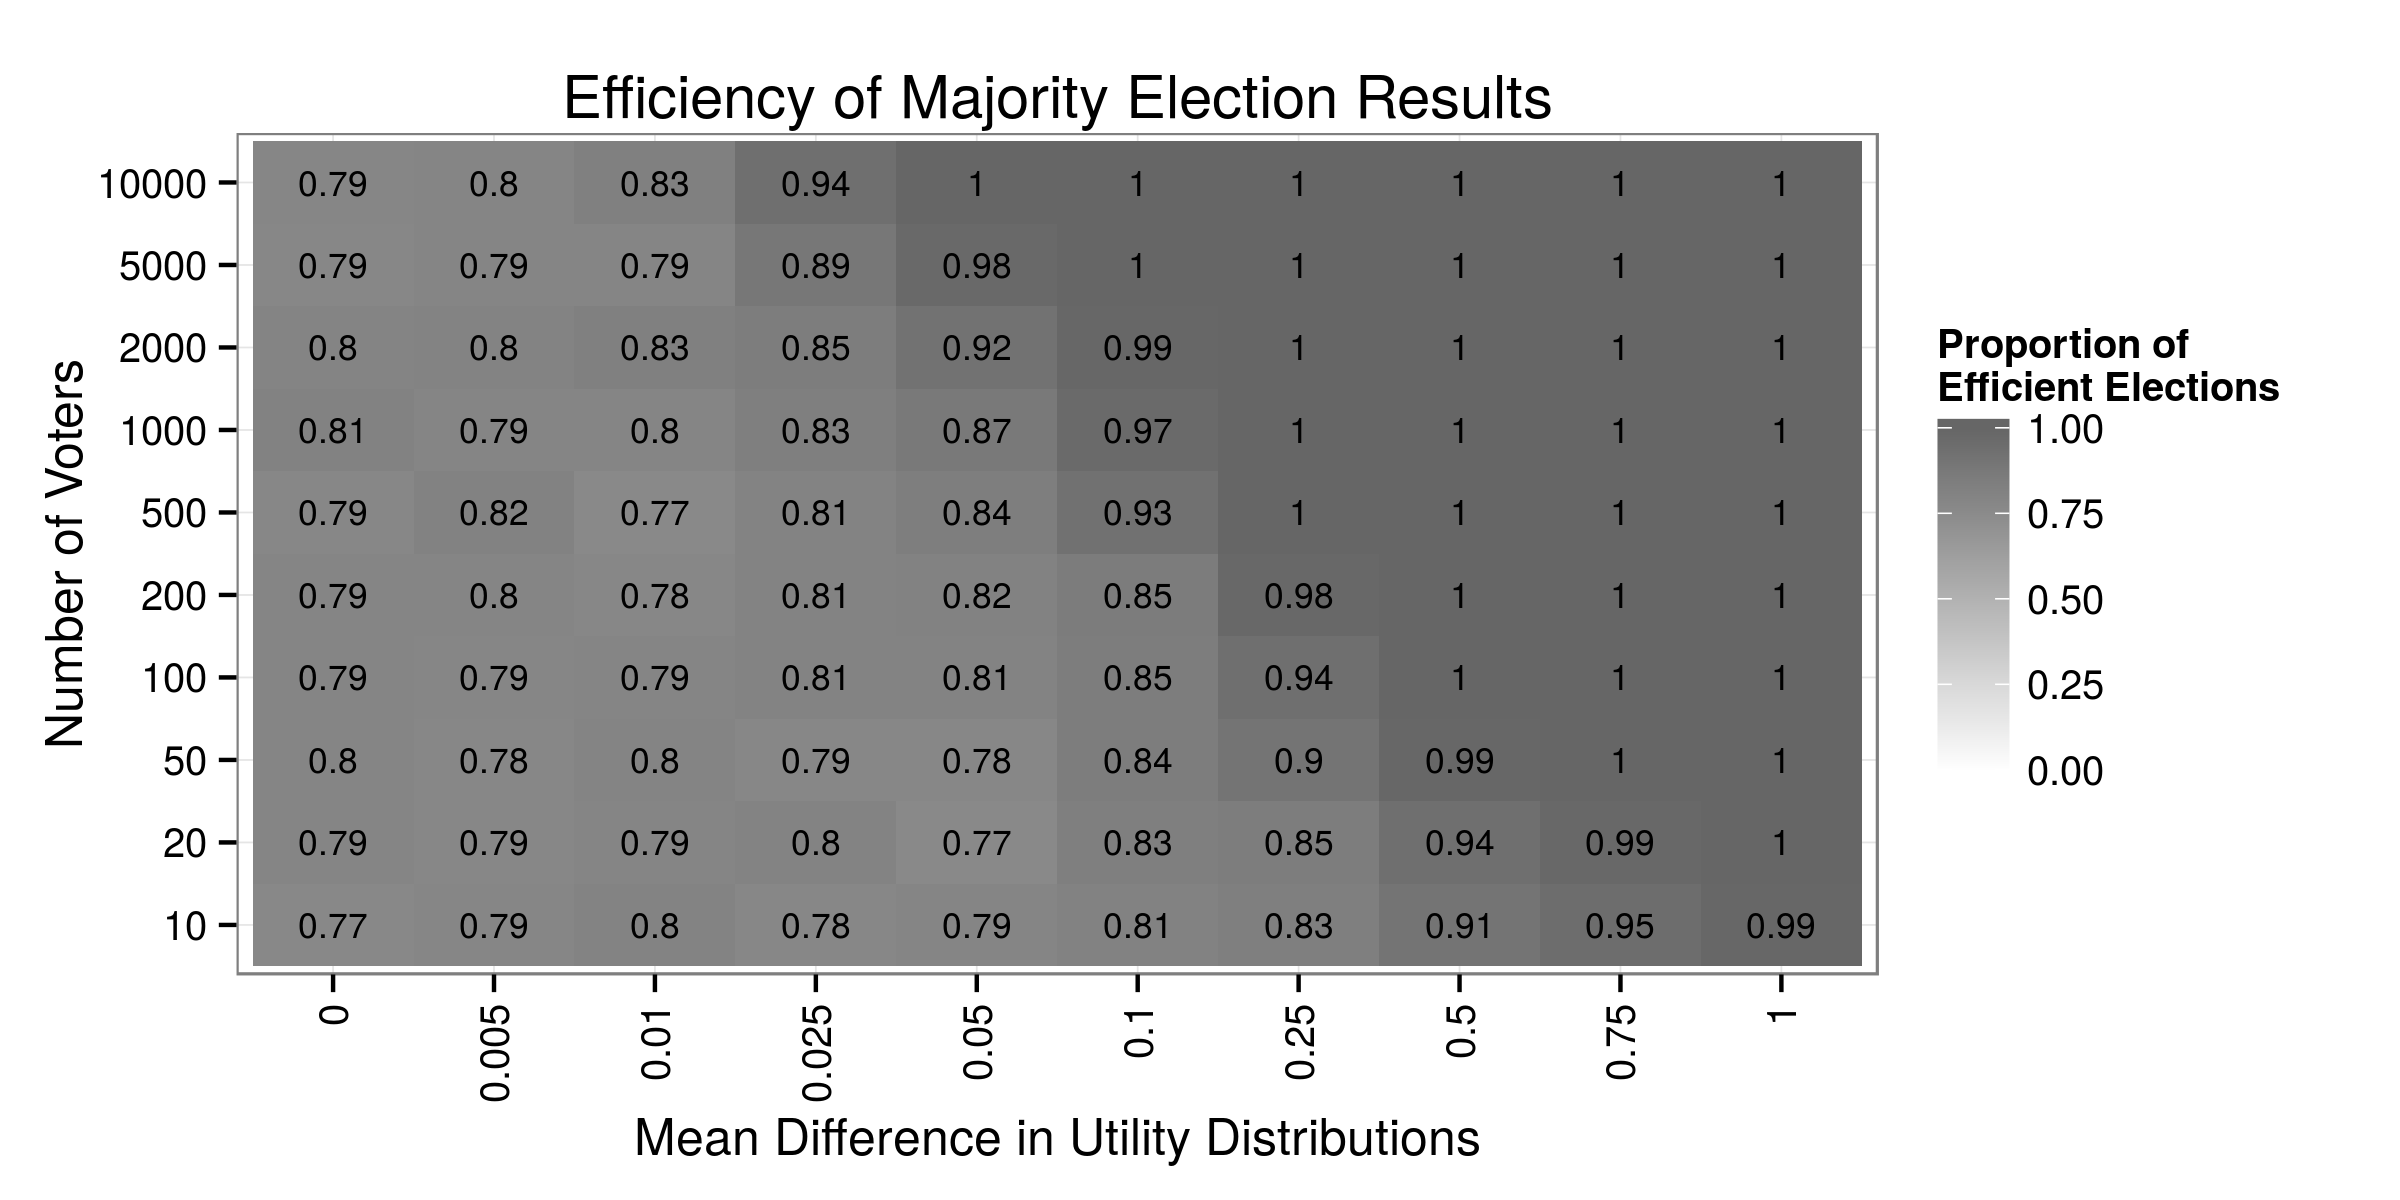
\includegraphics[height=.7\textheight]{../simulations/fig/s3b.png}
  \end{figure}
	$$ U_{i,A} \sim \mathcal{N}(\mu=0,\sigma^2=1) $$
        $$ U_{i,B} \sim \mathcal{N}(\mu=0+\epsilon,\sigma^2=1) $$
\end{frame}

\subsection{}
\begin{frame}%[allowframebreaks]
  \frametitle{Study 4: Skewed Policy Utilities I}
  \begin{figure}[ht]\centering
    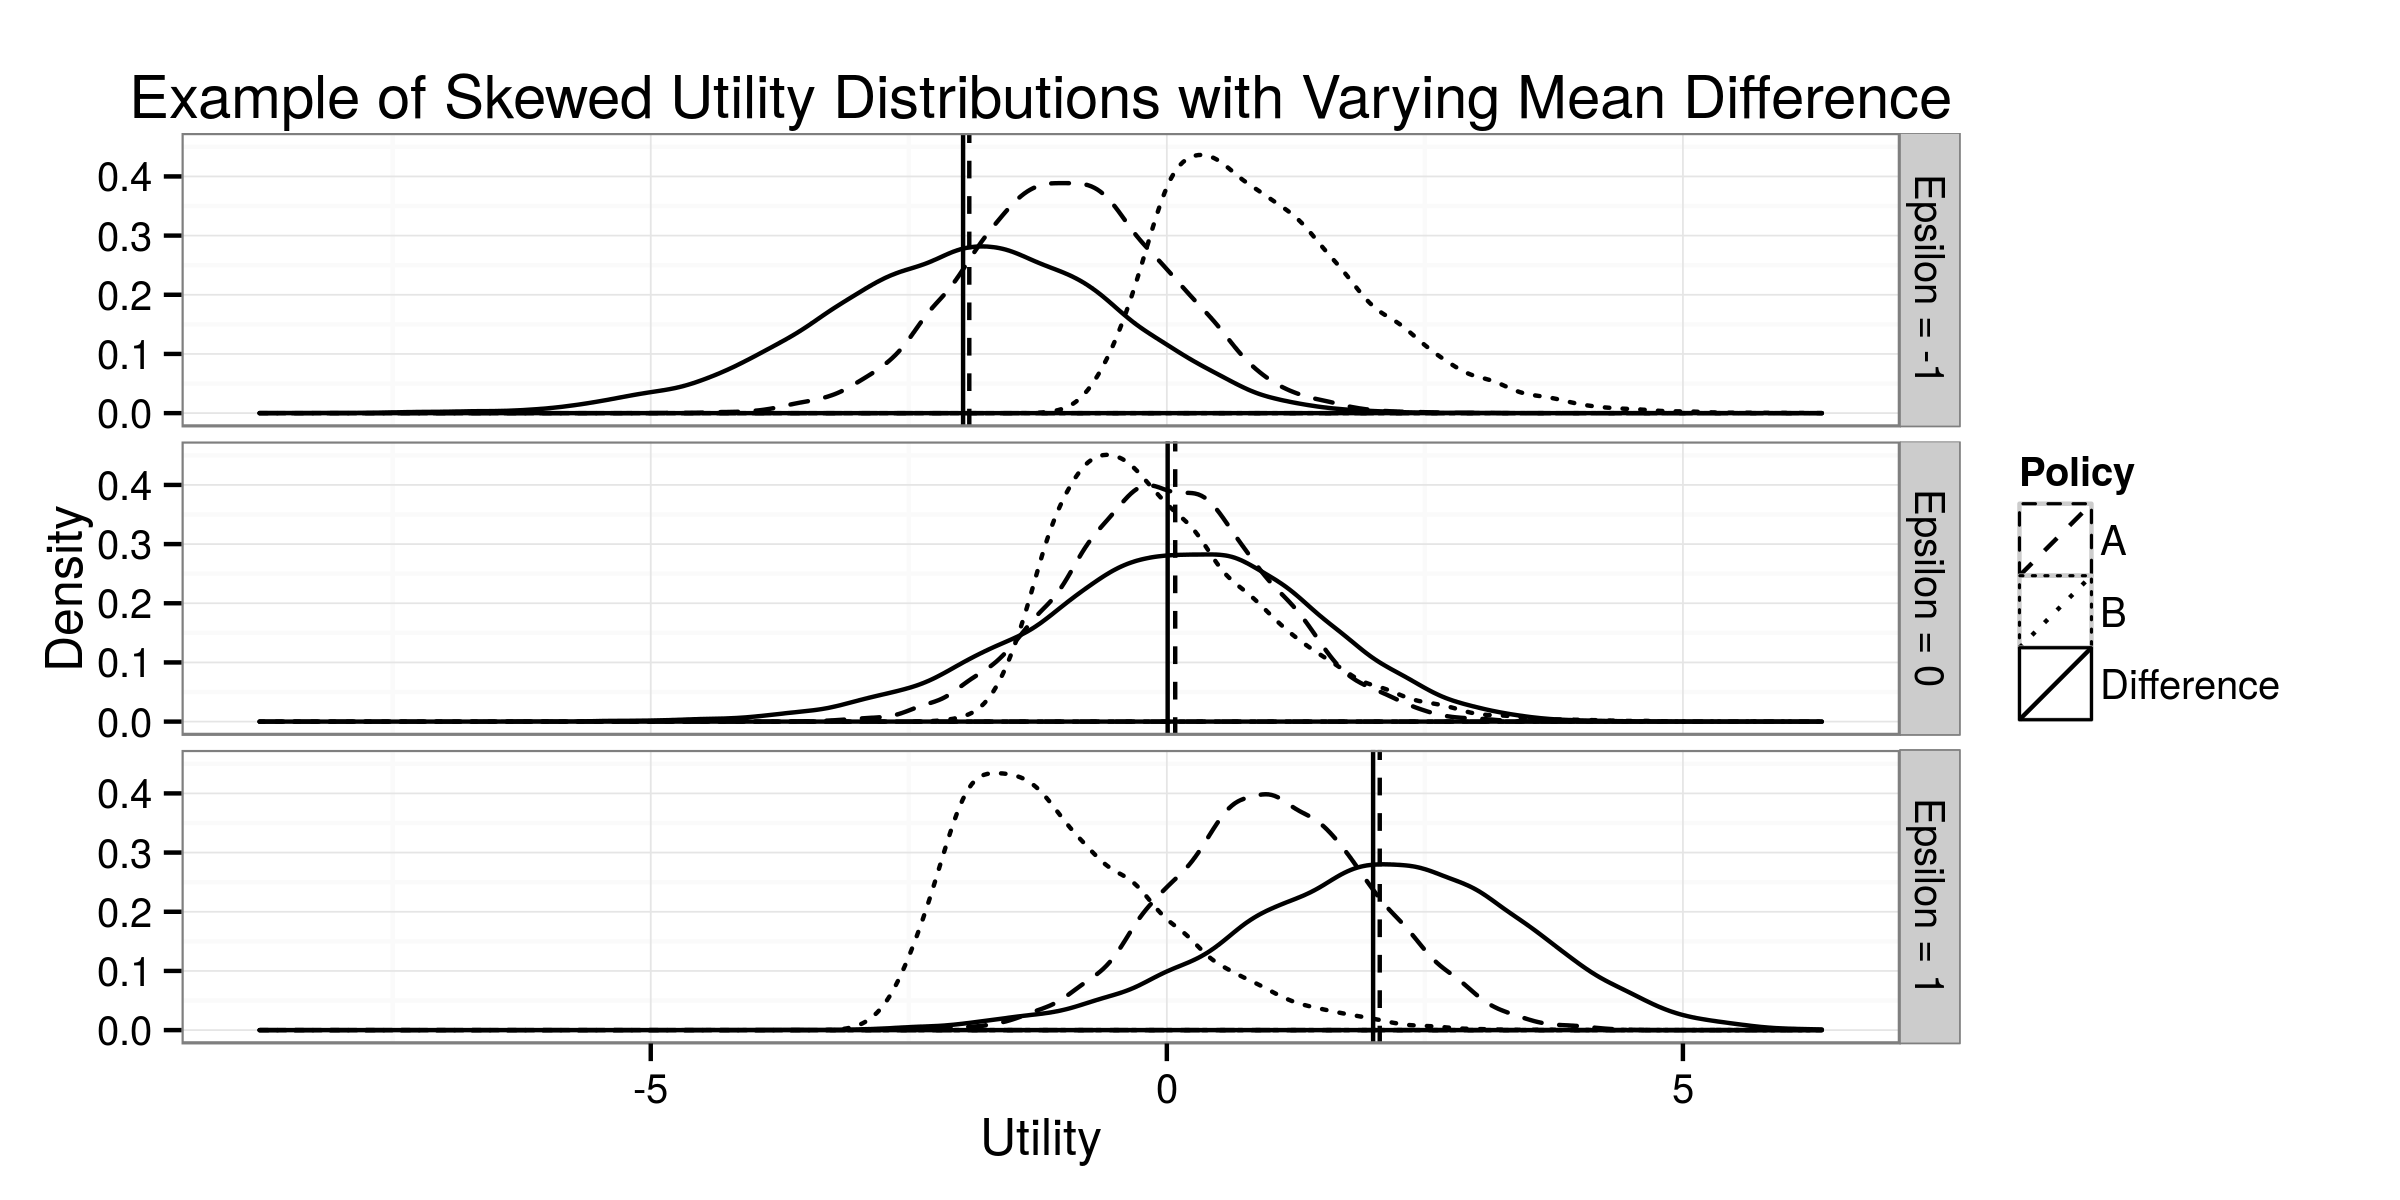
\includegraphics[height=.7\textheight]{../simulations/fig/s4a.png}
  \end{figure}
  	$$ U_{i,A} \sim \mathcal{N}(\mu=0+\epsilon,\sigma^2=1) $$
	$$ U_{i,B} \sim \mathcal{N}_\text{skew}(\mu=0-\epsilon,\sigma^2=1,\gamma=.85) $$
\end{frame}
\begin{frame}%[allowframebreaks]
  \frametitle{Study 4: Skewed Policy Utilities II}
  \begin{figure}[ht]\centering
    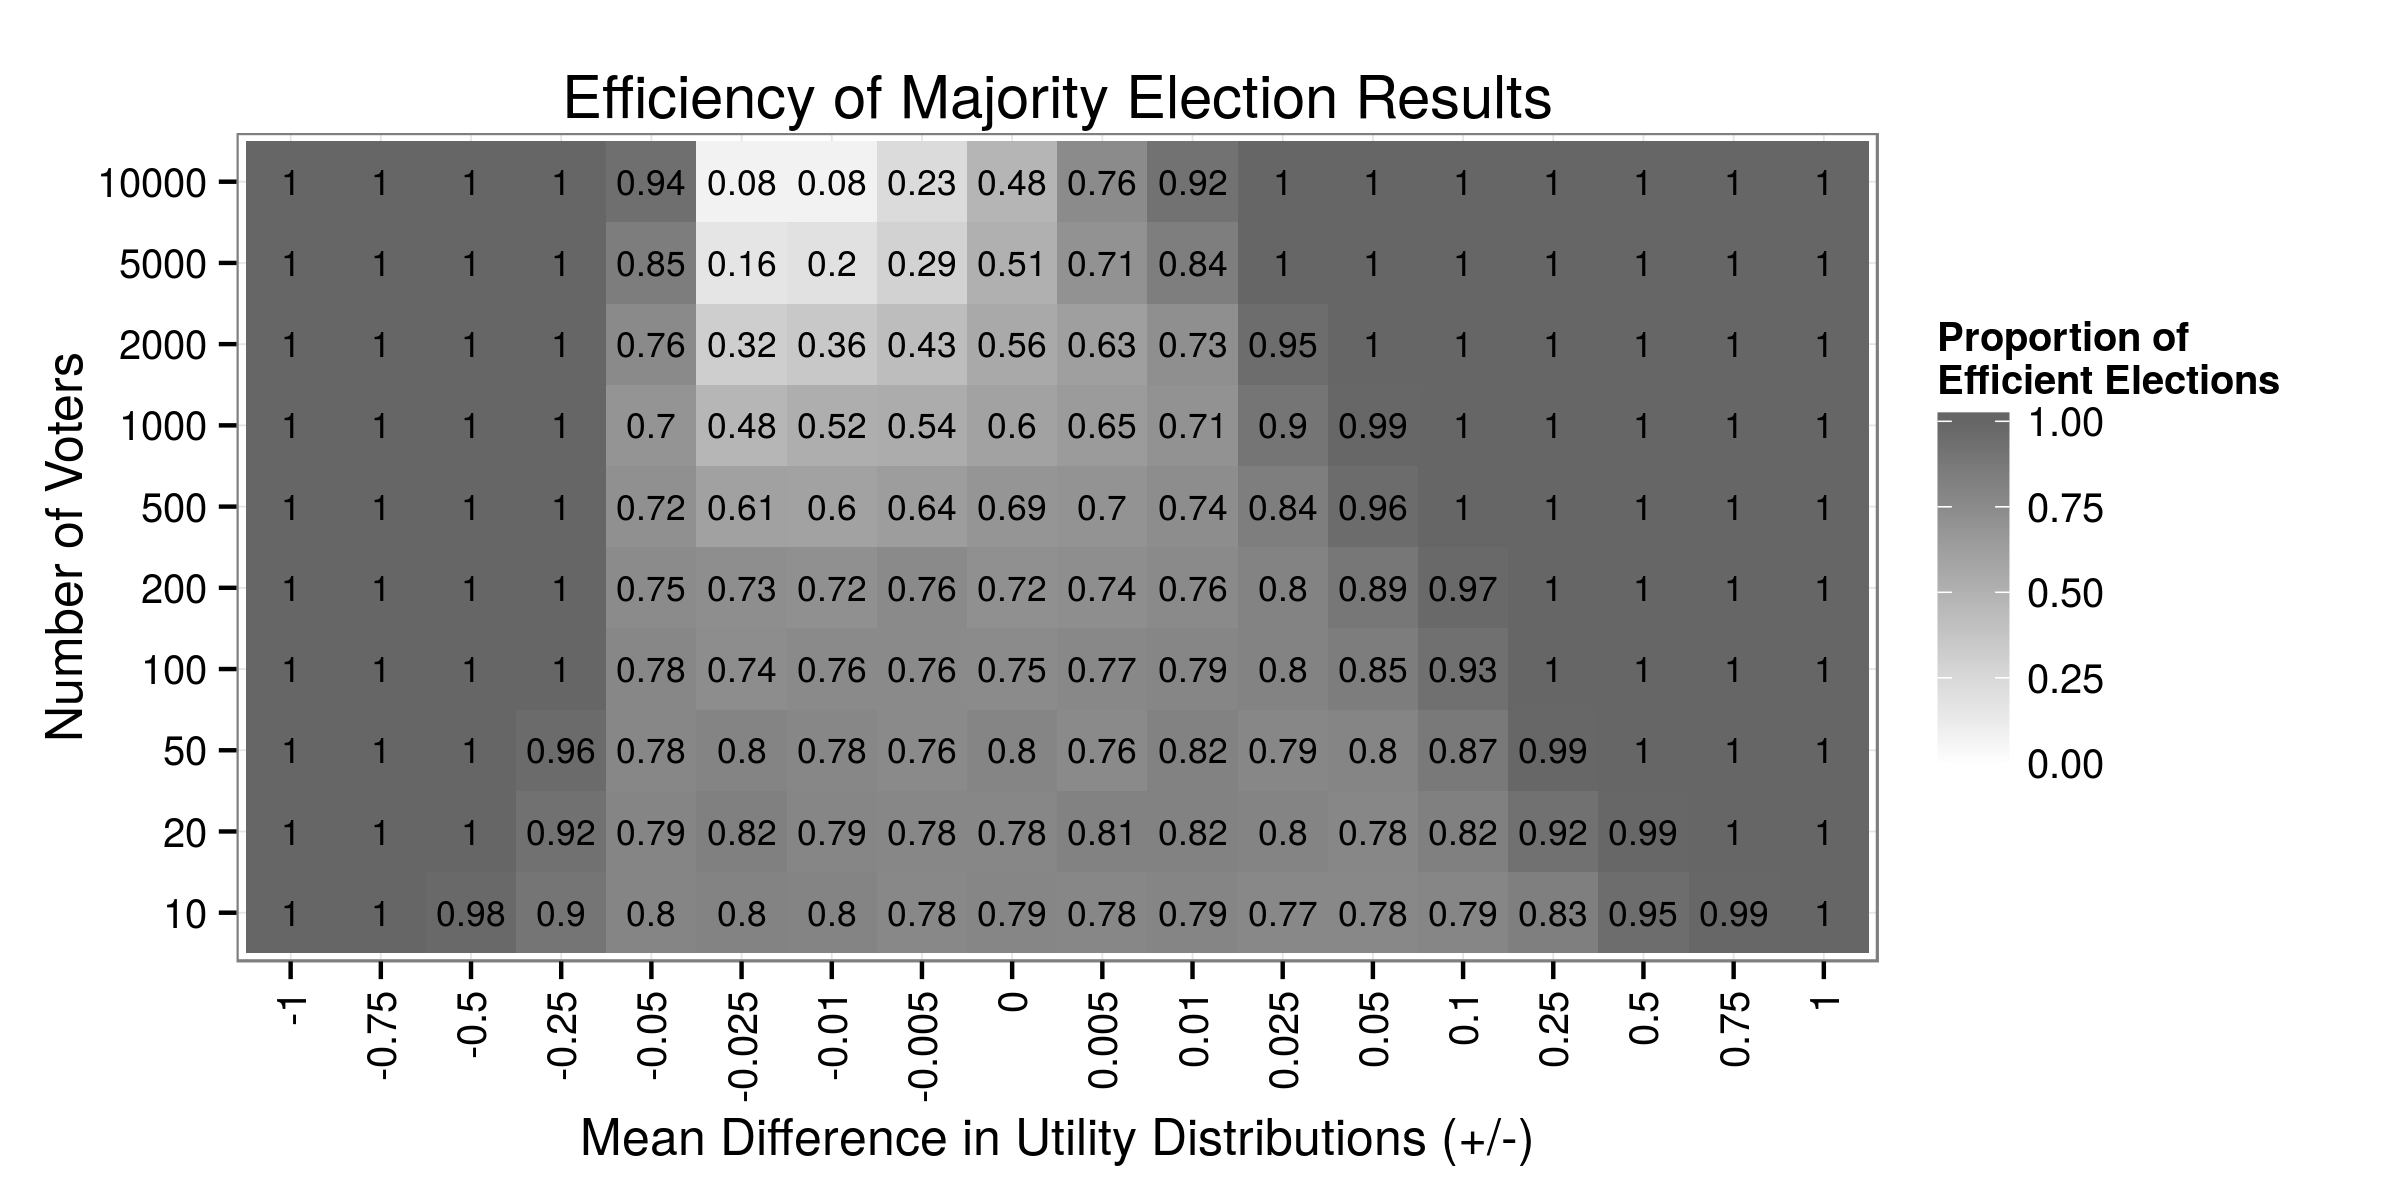
\includegraphics[height=.7\textheight]{../simulations/fig/s4b.png}
  \end{figure}
  	$$ U_{i,A} \sim \mathcal{N}(\mu=0+\epsilon,\sigma^2=1) $$
	$$ U_{i,B} \sim \mathcal{N}_\text{skew}(\mu=0-\epsilon,\sigma^2=1,\gamma=.85) $$
\end{frame}

\section{Discussion}
\subsection{}
\begin{frame}%[allowframebreaks]
  \frametitle{General Discussion}
  \begin{itemize}
    \item Efficiency of majority rule is contingent on assumptions/shape about voters' utilities
    \begin{itemize}
      \item \emph{aggregate difference} and \emph{skewness} of the distributions of individual utilities for each candidate affects the likelihood of inefficiencies
      \item under some scenarios, increasing the \emph{size of the electorate} actually reduces the efficiency of majority voting!
    \end{itemize}
    \item Spatial utilities might \emph{overestimate} efficiency due to (implicit) assumption of asymmetric policy positions

  \end{itemize}
\end{frame}

\subsection{}
\begin{frame}
  \frametitle{Further Developments}
    \begin{itemize}
      \item \emph{Additional scenarios}: vary number of policies, introduce uncertainty, vary decision rule etc.
      \item Consequences for \emph{political competition}
      \item Endogenous \emph{participation} and efficiency
      \item \emph{Experimental} designs
      \item Estimate \emph{likelihood for tyranny of the majority} in the context of actual political issues
    \end{itemize}
\end{frame}

\section{Appendix}
\subsection{}
\begin{frame}%[allowframebreaks]
  \frametitle{Study 2: Correlated Policy Utilities I}
  \begin{figure}[ht]\centering
    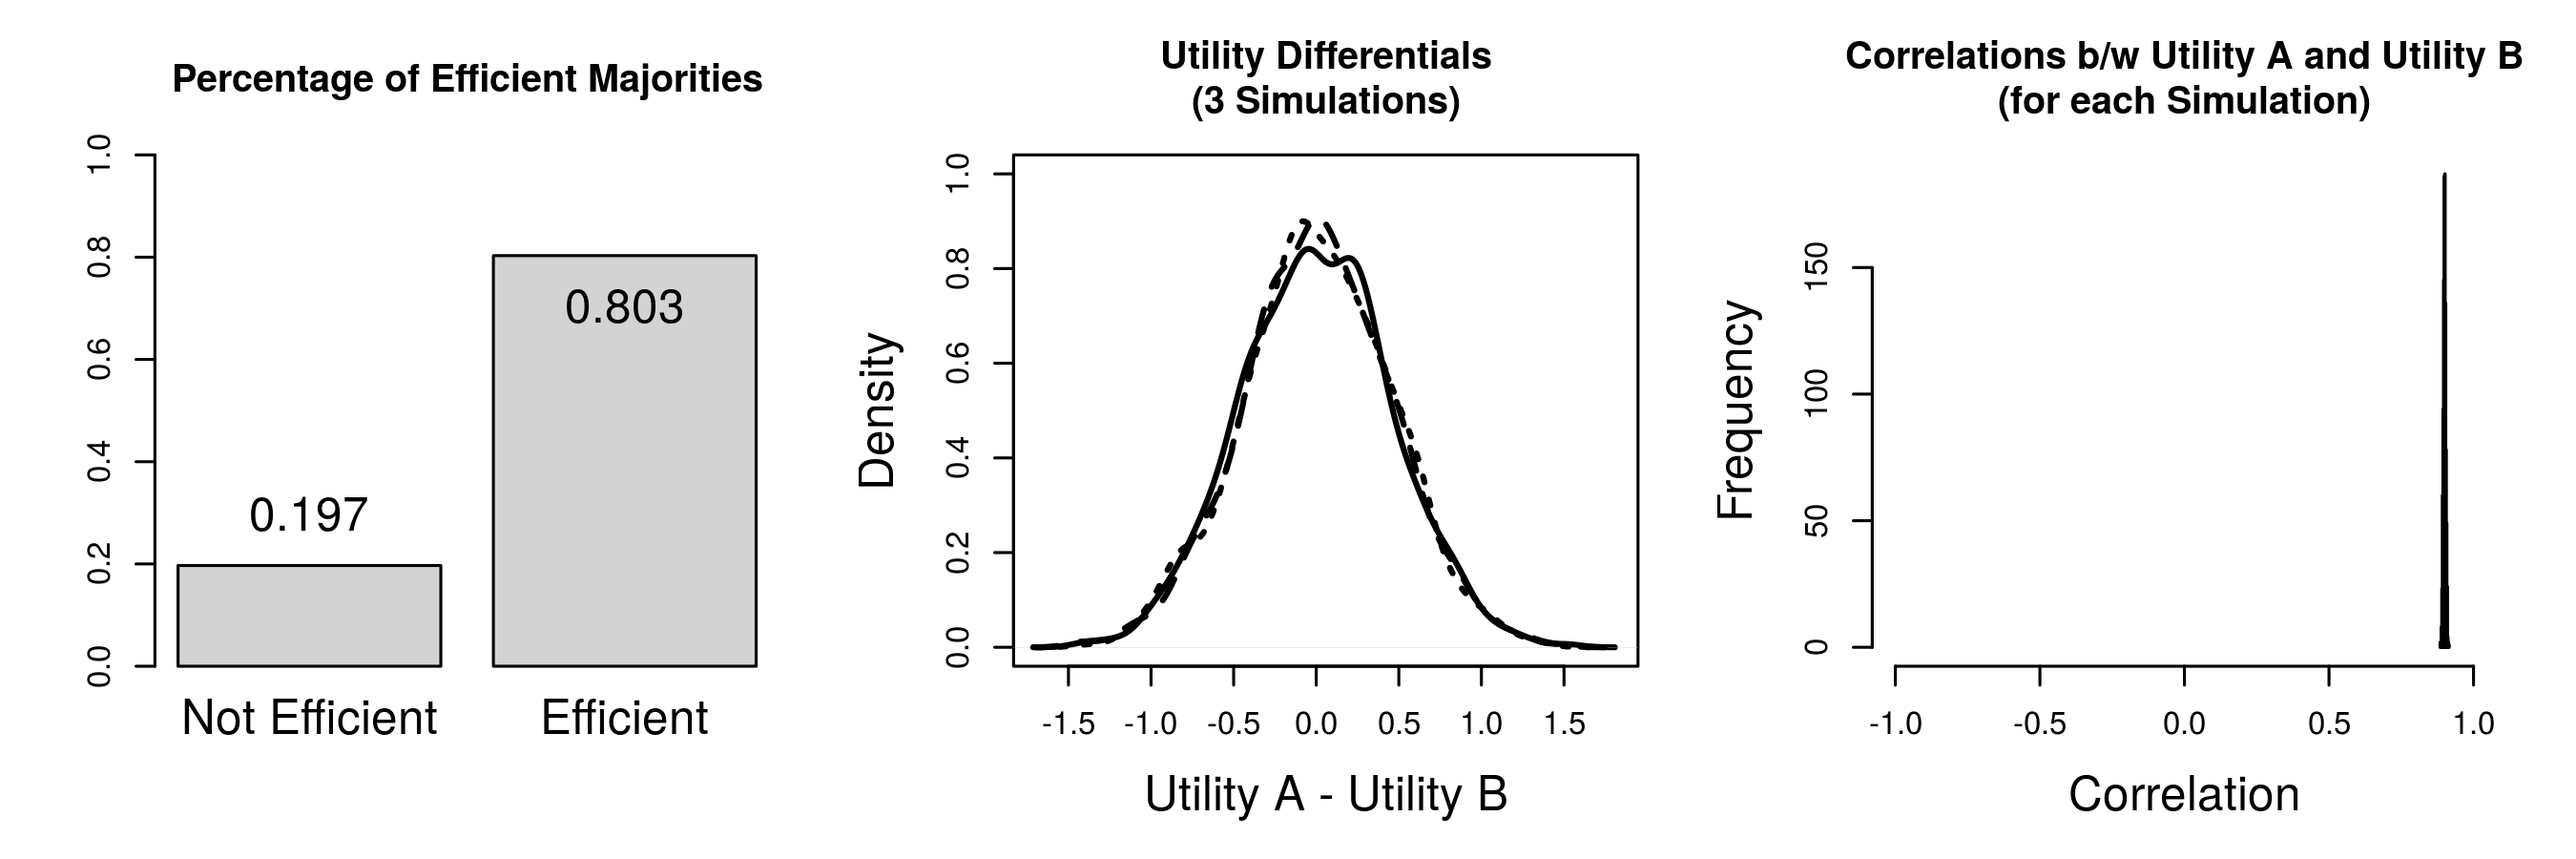
\includegraphics[width=\textwidth]{../simulations/fig/s2a.png}
    \caption{Positively correlated utilities}
  \end{figure}
  $$ \mathbf{U}_{i} \sim \mathcal{N}\left(
    \mathbf{\mu} =\begin{pmatrix}0 \\ 0\end{pmatrix},
    \mathbf{\Sigma} =\begin{pmatrix}1 & 0.9 \\ 0.9 & 1\end{pmatrix}
    \right) $$
\end{frame}
\begin{frame}%[allowframebreaks]
  \frametitle{Study 2: Correlated Policy Utilities II}
  \begin{figure}[ht]\centering
    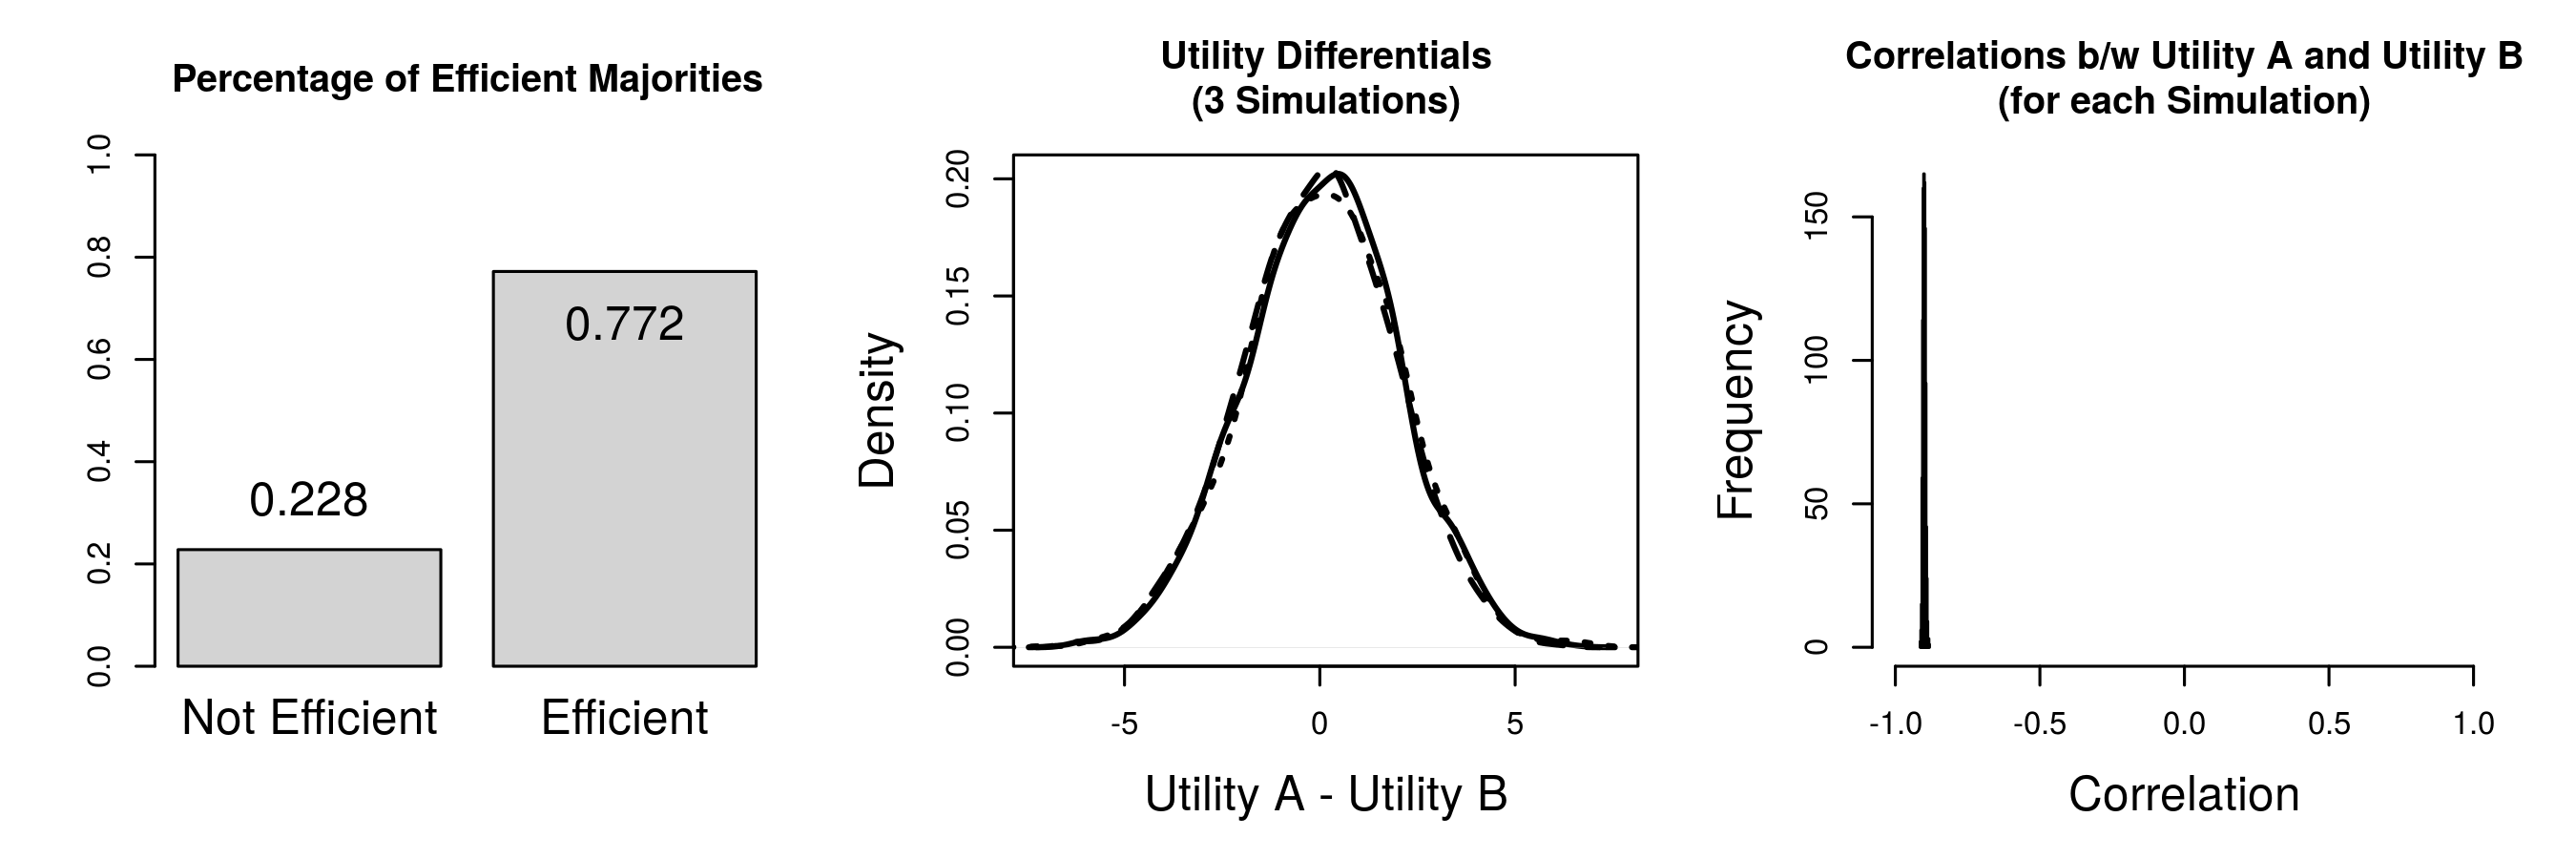
\includegraphics[width=\textwidth]{../simulations/fig/s2b.png}
    \caption{Negatively correlated utilities}
  \end{figure}
  $$ \mathbf{U}_{i} \sim \mathcal{N}\left(
    \mathbf{\mu} =\begin{pmatrix}0 \\ 0\end{pmatrix},
    \mathbf{\Sigma} =\begin{pmatrix}1 & -0.9 \\ -0.9 & 1\end{pmatrix}
    \right) $$
\end{frame}
\subsection{}
\begin{frame}%[allowframebreaks]
  \frametitle{Study 5: Inefficiencies with Spatial Utilities I}
  \begin{figure}[ht]\centering
    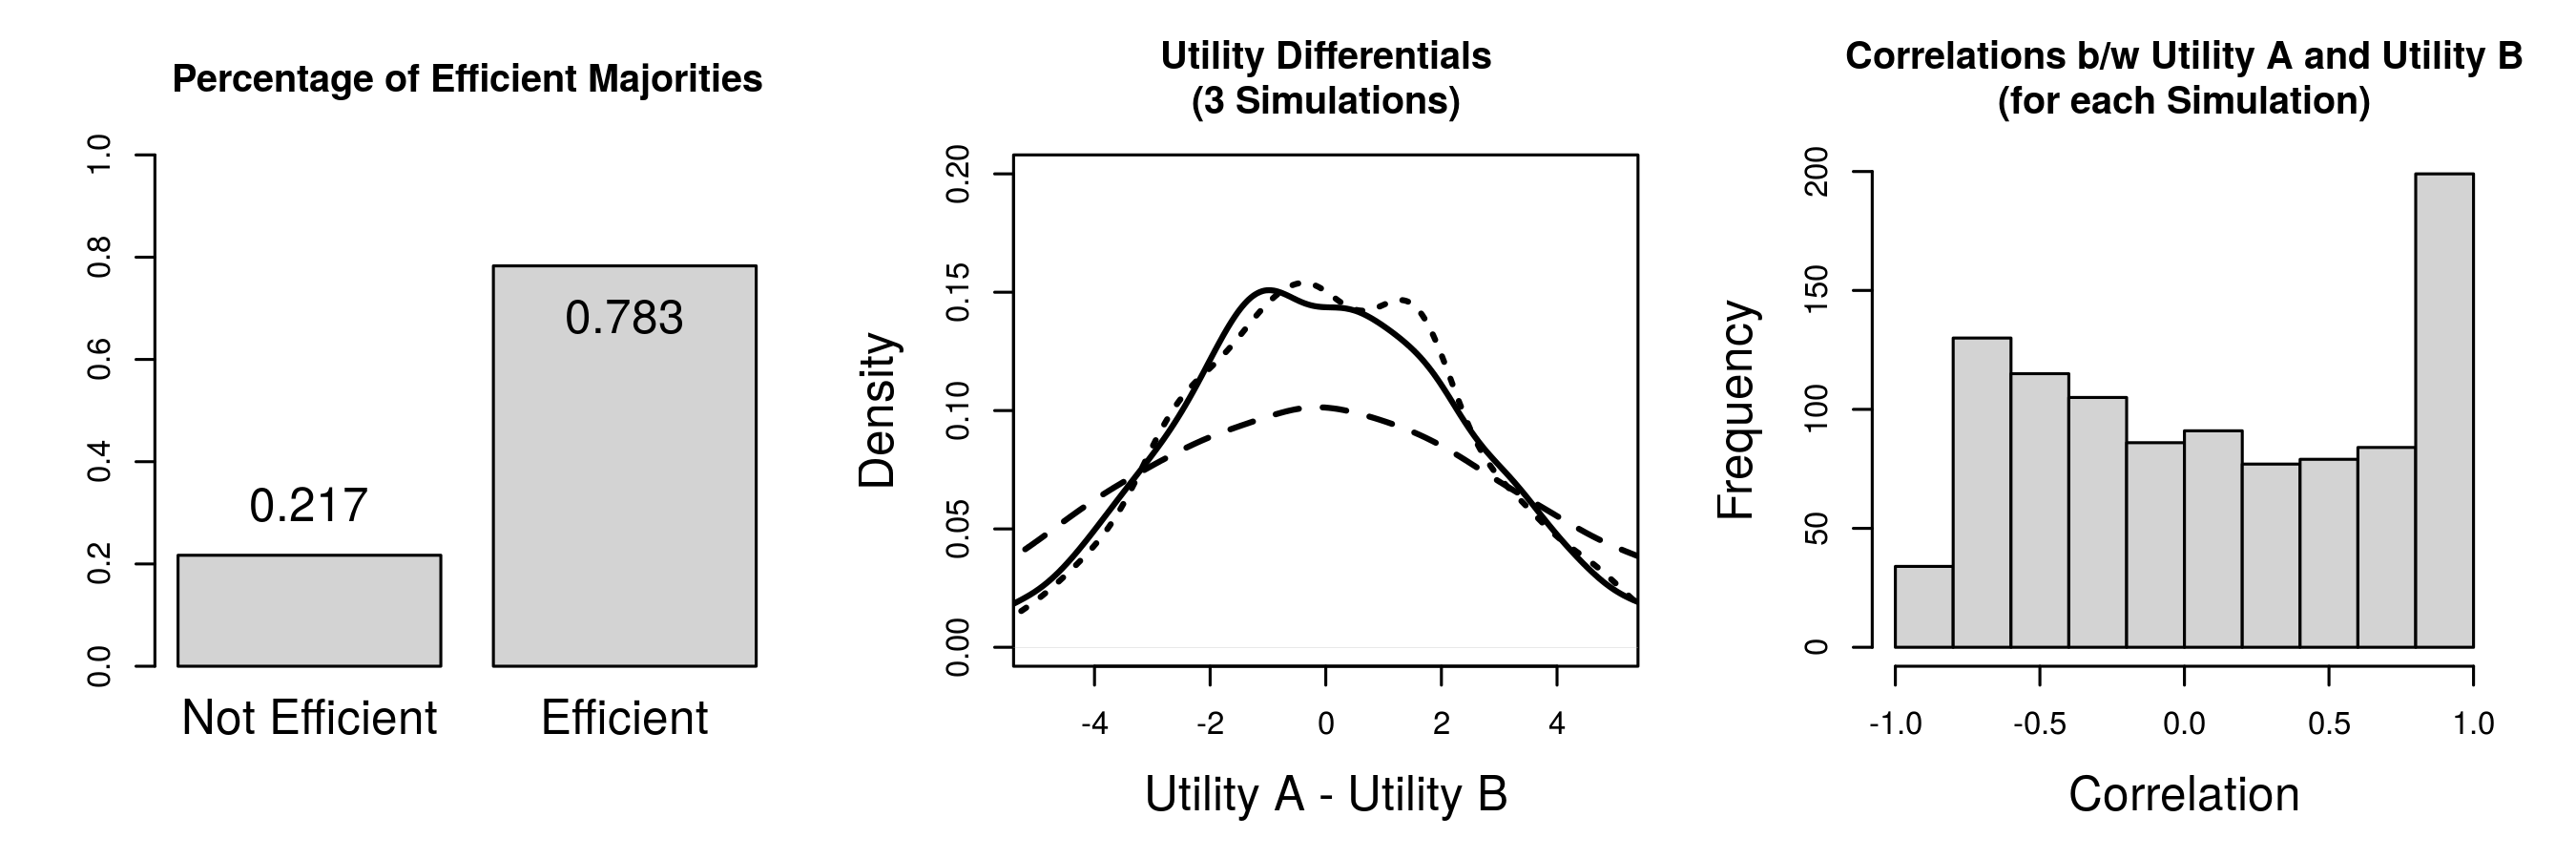
\includegraphics[width=\textwidth]{../simulations/fig/sX2.png}
    \caption{Symmetric policy positions}
  \end{figure}
	$$ V_i,P_{A} \sim \mathcal{N}(\mu=0,\sigma^2=1) \hspace{1cm} P_{B} = -1*P_{A} $$
	$$ U_{ij} = -(V_i - P_j)^2 $$
\end{frame}
\subsection{}
\begin{frame}%[allowframebreaks]
  \frametitle{Study 5: Inefficiencies with Spatial Utilities II}
  \begin{figure}[ht]\centering
    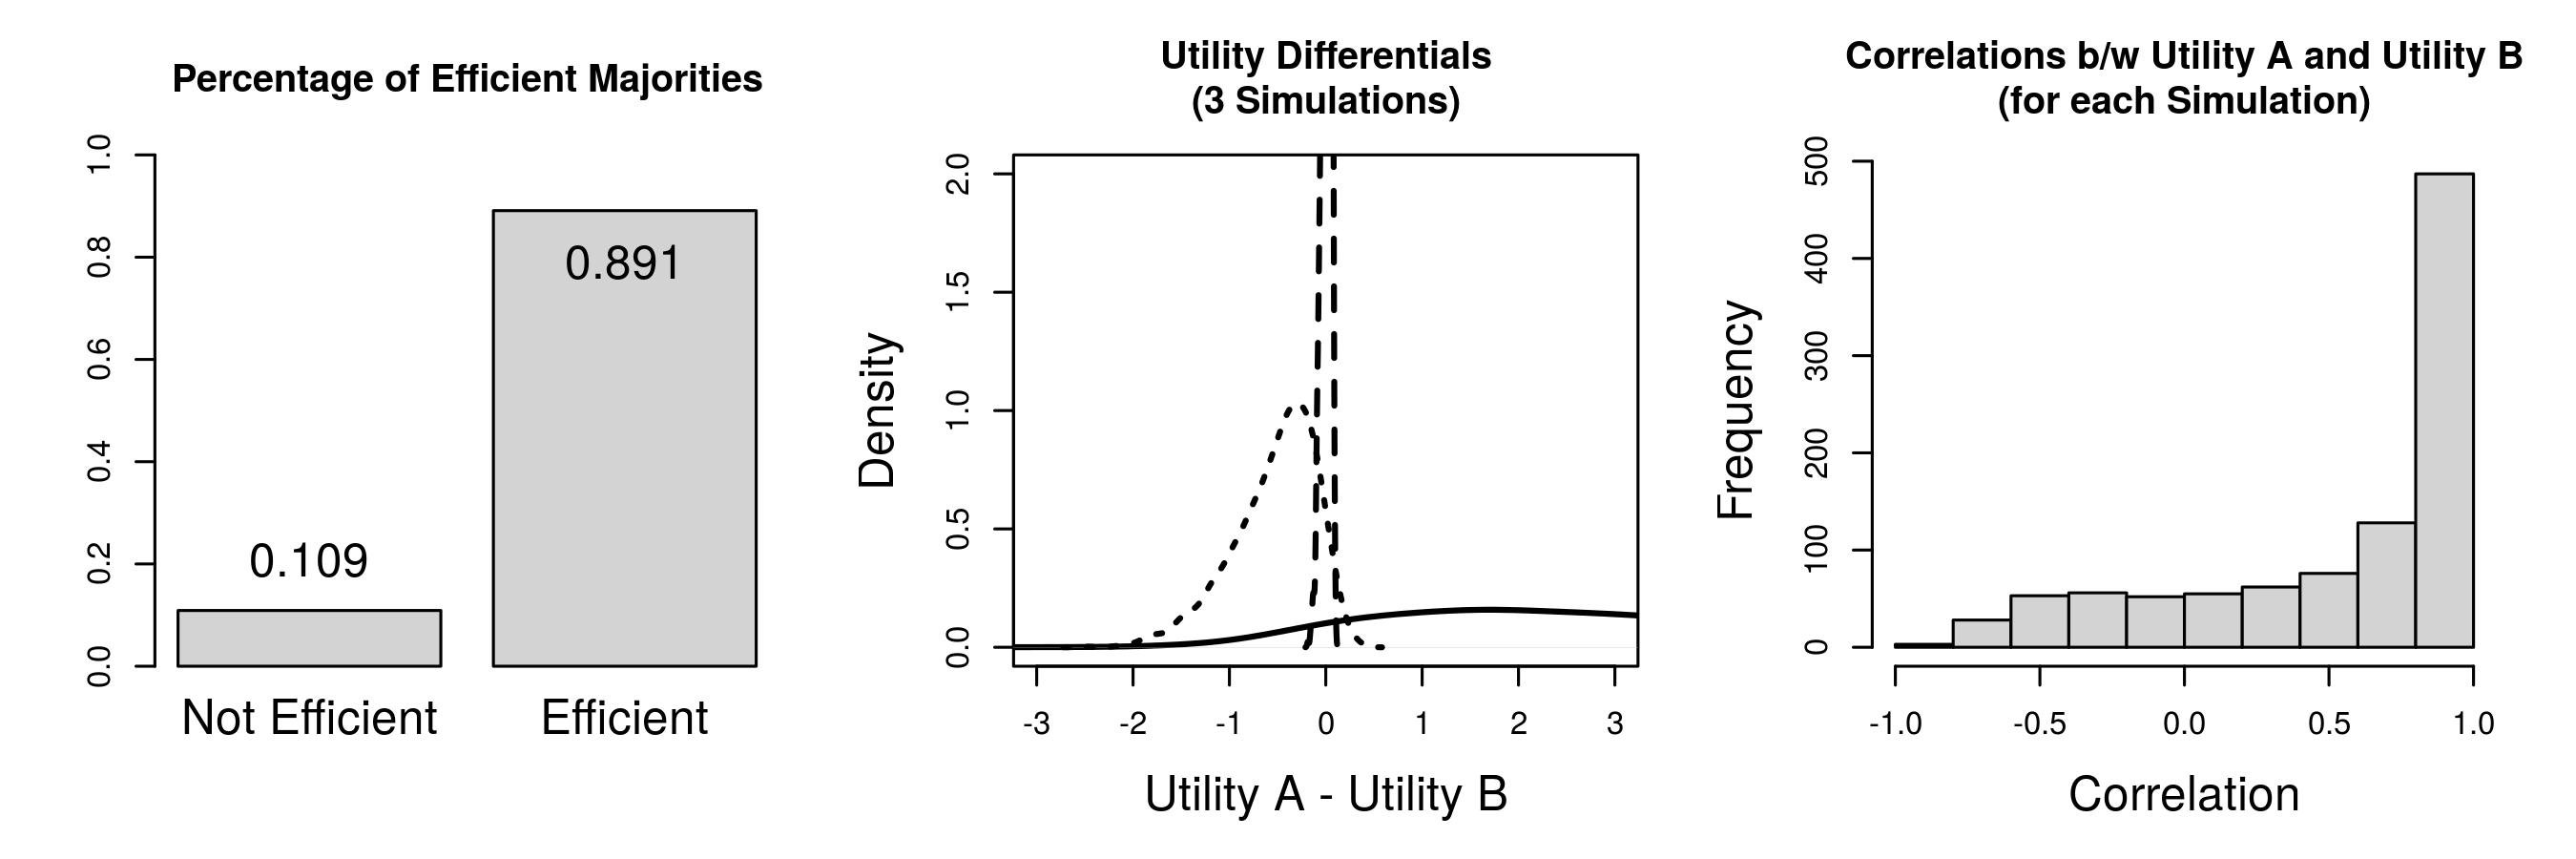
\includegraphics[width=\textwidth]{../simulations/fig/sX1.png}
    \caption{Skewed ideal points}
  \end{figure}
	$$ V_i \sim \mathcal{N}_\text{skew}(\mu=0,\sigma^2=1,\gamma=.85) \hspace{1cm} P_j \sim \mathcal{N}(\mu=0,\sigma^2=1) $$
	$$ U_{ij} = -(V_i - P_j)^2 $$
\end{frame}

\subsection{}
\begin{frame}
  \frametitle{References}
  \def\newblock{\hskip .11em plus .33em minus .07em}
  %\nocite{*}
  \begin{scriptsize}
    \bibliographystyle{apsr}
    \bibliography{/data/Copy/1-src/lit/Literature}
  \end{scriptsize}
\end{frame}

\end{document}